\documentclass{article}[12pt]
\usepackage[a4paper, margin=1in]{geometry}
\usepackage[utf8]{inputenc}
\usepackage[english]{babel}
\usepackage{amssymb, amsmath, amsthm} % math symbols
\usepackage{csquotes} % format quote blocks
\usepackage{hyperref} % hyperlinks
\usepackage[table]{xcolor} % tables
\usepackage{graphicx}

\hypersetup{
    colorlinks=true,
    linkcolor=black,
    citecolor=black,
    urlcolor=blue,
    pdfborderstyle={/S/U/W 1}
    }

% title
\title{Learning Notation: Seminar Two \\ Set Theory}
\author{Jack (Quan Cheng) Xie}
\date{\today}
    
% % margin spacing
% \oddsidemargin 3mm
% \evensidemargin 3mm
% \topmargin -12mm
% \textheight 600pt
% \textwidth 420pt

% paragraph /indent spacing
\setlength{\parskip}{6pt}
\setlength{\parindent}{0pt}


% mathtools equation numbering
\counterwithin*{equation}{section}
\renewcommand\theequation{\thesection.\arabic{equation}}

% amsthm theorems formatting
\newtheorem{theorem}{Theorem}

\newtheorem{conjecture}{Conjecture}
\newtheorem*{conjecture*}{Conjecture} % unnumbered

\newtheorem{proposition}{Proposition}
\newtheorem*{proposition*}{Proposition} 

\newtheorem{claim}{Claim}
\newtheorem*{claim*}{Claim}

\newtheorem{definition}{Definition}
\newtheorem*{definition*}{Definition} % unnumbered

\newtheorem{exercise}{Exercise}
\newtheorem*{exercise*}{Exercise} % unnumbered


% special symobls
\newcommand{\N}{\mathbb{N}}
\newcommand{\Z}{\mathbb{Z}}
\newcommand{\Q}{\mathbb{Q}}
\newcommand{\R}{\mathbb{R}}
\newcommand{\C}{\mathbb{C}}
\newcommand{\PS}{\mathcal{P}}

% text box for definitions and theorems
\newcommand{\textbox}[1]{\fbox{\parbox{\textwidth}{#1}}}

% bibliography formatting
\makeatletter
\renewcommand{\@biblabel}[1]{$\triangleright$}
\makeatother

\begin{document}

    \maketitle
        
    \section{Sets and Membership}
        
        \subsection{Elements and membership}
            
            \textbox{
                \begin{definition}[Naive set]
                    \label{def:inf-function}
                        A \textbf{set} is an unordered collection of unique objects. The objects in a set are called its \textbf{elements.}
                \end{definition}
            }
            
            For example, if some unique variables $a, b, c$ are the elements of the set $S$, we can write
            \begin{equation}
                S = \{a, b, c\}. \label{abc-set}
            \end{equation}
            Then $a, b, c$ are elements of $S$, which we can express as
            \begin{equation}
                a, b, c \in S. \label{abc-elements}
            \end{equation}
            The ``$\in$" symbol is read ``is an element of" or ``are elements of." We can also say that $a, b, c$ are \textbf{members} of $S$, $a, b, c$ \textbf{belong} to $S$, and $S$ \textbf{contains} $a, b,$ and $c$.
            If $S = \{a, b, c\}$, then for some other unique element $d$ not in the set, we can write
            \begin{equation}
                d \notin S = \{a, b, c\}.
            \end{equation}
            The elements of a set must be \textbf{unique}, meaning a set cannot contain more than one of the same thing. For example, it would be slightly improper to write
            \begin{equation}
                S = \{a, a, b, c\},
            \end{equation}
            since the element $a$ is not unique in $S$. Alternatively, we can say that
            \begin{equation}
                \{a, a, b, c\} = \{a, b, c\},
            \end{equation}
            by ignoring the repeated element $a$.
        
            \begin{exercise}
                For a set $A$, does $a_1, a_2, a_3 \in A$ imply $A = \{a_1, a_2, a_3\}?$
            \end{exercise}
            
            
        \subsection{Set equality and element order}
            
            Two sets are \textbf{equal} if they have the same elements, regardless of the order of the elements. For example,
            \begin{equation}
                \{a, b, c\} = \{c, b, a\}.
            \end{equation}
            
        \subsection{Cardinality}
            
            A set is \textbf{infinite} if it has infinitely many members. Otherwise it is \textbf{finite.} For example, the set
            \begin{equation}
                \{0, 1, 2, 3, ...\}, \label{naturals}
            \end{equation}
            which contains all natural numbers (non-negative integers) is infinite. The \textbf{cardinality} or \textbf{size} of a set is the number of elements it has. For a set $S$, we write its cardinality as $|S|.$ For example, if $S = \{a, b, c\}$ then
            \begin{equation}
                |S| = |\{a, b, c\}| = 3.
            \end{equation}
            Two sets are \textbf{equicardinal} if they have the same cardinality. For example, if
            \begin{align}
                A = \{1, 2, 3, 4, 5\}, \quad B = \{3, 4, 5, 6, 7\},
            \end{align}
            then $|A| = |B| = 5$, so $A$ and $B$ are equicardinal. This is a very informal definition of cardinality. We will look at a more formal definition of equicardinality when discussing functions.
            
        \subsection{Empty set, sets as elements}
        
            The \textbf{empty set} is a special set that contains no elements. We denote it by $\varnothing$ or $\{\}$. A set can have other sets as its members. For example, the following are valid sets:
            \begin{align}
                A &= \{a, b, c\}, \quad B = \{1, 2, 3\},
                \\
                C &= \{\varnothing, A, B\} = \{\{\}, \{a, b, c\}, \{1, 2, 3\}\},
                \\
                D &= \{\varnothing, a, b, c, 1, 2, 3, C\}
                = \{\{\}, a, b, c, 1, 2, 3, \{\{\}, \{a, b, c\}, \{1, 2, 3\}\}\}.
            \end{align}
            
            \begin{exercise}
                What are $|D|$, $|\varnothing|$, and $|\{\varnothing\}|$?
            \end{exercise}
        
        \subsection{Number systems}
            
            We've seen the empty set $\varnothing$, which is a special concept in set theory. Now we will look at some other commonly used sets and their conventional notation. These are $\N, \Z, \Q,$ and $\R$, which are the sets of natural, integer, rational, and real numbers.
            
            The set of \textbf{natural numbers}, which has only positive whole number elements (and zero), is denoted as
            \begin{equation}
                \N = \{0, 1, 2, 3, ...\}.
            \end{equation}
        
            The set of \textbf{integers}, which contains all positive and negative whole numbers and zero, is denoted as
            \begin{equation}
                \Z = \{0, 1, -1, 2, -2, ...\}.
            \end{equation}
            
            The set of \textbf{rational numbers}, which contains all integers that can be written as a fraction of integers, is denoted as
            \begin{equation}
                \Q
                = \left\{..., -\frac{1}{1} , \frac{0}{1}, \frac{1}{1}, \frac{1}{2}, \frac{2}{1}, \frac{1}{3}, \frac{3}{1}, \frac{1}{4}, \frac{2}{3}, \frac{3}{2}, \frac{4}{1}, ...\right\}
            \end{equation}
            
            The set of \textbf{real numbers} is written as
            \begin{align}
                \R
                &= (-\infty, \infty), \label{reals-interval}
            \end{align}
            which contains numbers like $\pi, e,$ and $\sqrt{2}$ that cannot be expressed as fractions of integers.
            
            \textbox{
                \begin{proposition}
                    The number $\sqrt{2}$ is irrational.
                \end{proposition}
            }
            \begin{proof}
                By contradiction, suppose that $\sqrt{2}$ is rational. Then there exists $p, q \in \Z$ with no common factors where $\sqrt{2} = \frac{p}{q}$. Then we have that
                \begin{align*}
                    \sqrt{2} = \frac{p}{q}
                    & \implies
                    2 = \frac{p^2}{q^2} \\
                    & \implies
                    p^2 = 2 p^2.
                \end{align*}
                Since $p$ is an integer, then $p$ must be divisible by 2, thus $p = 2m$ for some $m \in \Z$. Then we have that \begin{align*}
                    2 q^2 = p^2, p = 2m
                    & \implies
                    2 q^2 = 4m^2 \\
                    & \implies 
                    q^2 = 2m^2.
                \end{align*}
                Since $q$ is also an integer, it must also be divisible by 2. Then both $p$ and $q$ are divisible by two, which contradicts the statement that they have no common factors.
            \end{proof}
            
            We also have the set of complex numbers, denoted by $\C$, which can be constructed from all pairs of real numbers $x, y \in \R$. We have $x$ for the real component, and add it to $y$ times $i = 
            \sqrt{-1}$, the imaginary component. We can write the complex numbers using set builder notation:
            \begin{align}
                \C
                &= \left\{ x + y i \; : \; x, y \in \R, \; i = \sqrt{-1} \label{complex} \right\}
            \end{align}
            
            \begin{exercise}
                Show that $\sqrt{3}$ is irrational.
            \end{exercise}
            
        \subsection{Set builder notation}
            
            Up to now we have mostly been explicitly writing sets with \textbf{set roster notation}. The can be a little vague if we are not careful\footnote{Think bout how would you explicitly write the members of $\R$? How could you tell it apart from $\Q$?}. Instead we can use \textbf{set builder notation} to precisely specify what elements we want in a defined set. For example, we can write the set of all positive real numbers $\R$ as
            \begin{equation}
                (0, \infty) = \{x \in \R : x > 0\}. \label{R-plus}
            \end{equation}
            
            We sometimes call this set $\R^+$. The ``$:$" symbol can be read \textbf{``where"} or \textbf{``such that."} Sometimes we use ``$|$" instead of ``$:$". The right hand side of \eqref{R-plus} is read, "the set of all elements $x$ in the reals where $x$ is greater than zero."
            
            \begin{exercise}
                Construct $\Z$ and $\Q$ from $\N$ with set builder notation.
            \end{exercise}
        
        \subsection{Tuples and Cartesian product}
        
            
            \textbox{
            \begin{definition}[Tuple]
                Informally, a \textbf{tuple} is a finite, ordered list (or sequence) of elements. A \textbf{n-tuple} is a tuple of $n$ elements.
                \begin{align}
                    (a_1, a_2, a_3, ..., a_n).
                \end{align}
            \end{definition}
            
            \begin{definition}[Cartesian product]
                The \textbf{Cartesian product} of two sets $A$ and $B$ is the set of all pairs (or 2-tuples) of elements $(a, b)$ from $a \in A$ and $b \in B$.
                \begin{align}
                    C = A \times B = \{(a, b) : a \in A, b \in B\}
                \end{align}
                
                We can generalize to the definition of a $n$-ary Cartesian product of arbitrary many sets:
                \begin{align}
                    X_1 \times ... \times X_n
                    = \{(x_1, ..., x_n) : x_i \in X_i, \forall i \in \{i, ..., n\}\}
                \end{align}
            \end{definition}
            }
            
        \subsection{Russell's paradox}
        
            So far we have allowed pretty much anything to be a member of a set, including other sets. However, if we are not careful with our formulation of what sets are, we can run into some problems. The logician Bertrand Russell came up with a famous problem that arises from loose definitions of sets.
            
            \textbox{
                \begin{proposition}[Russell's paradox]
                    Let $R = \{S : S \not\in S\}$, the set of all sets that are not members of themselves. Then $R \in R \iff R \not\in R$.
                \end{proposition}
            }
            \begin{proof}
                We have that $R \in R \implies R \not\in R$, since if $S = R \in R$, then by its membership in $R$ it must satisfy the condition of being a set $S \not\in S$ that is not a member of itself, which means $R \not\in R$.
                \\
                
                We have that $R \not\in R \implies R \in R$ by the definition of the set $R$. If $R$ is not a member of itself, then it must be a member of ``the set of all sets that are not members of itself," which is $R$.
            \end{proof}
        
            To resolve such paradoxes, mathematicians limit what are allowed to be valid sets, which is standardized with the \href{https://en.wikipedia.org/wiki/Zermelo\%E2\%80\%93Fraenkel_set_theory}{Zermelo-Fraenkel axioms} (ZF axioms). However, problems with naive set theory apparently rarely come up unless you specifically look for them, like the case of Russell's paradox.
            
        
    \section{Set Operations and Subsets}
    
        \subsection{Union}
            \textbox{
                \begin{definition}[Union]
                    The \textbf{union} of sets $A$ and $B$ are defined as
                    \begin{align}
                        A \cup B = \{ x : (x \in A) \lor (x \in B) \}.
                    \end{align}
                \end{definition}
            }
            
            For example, if $A = \{a, b, c\}$ and $B = \{b, c, d, e\}$ then $A \cup B = \{a, b, c, d, e\}$.
            
        \subsection{Intersection}
            \textbox{
                \begin{definition}[Intersection]
                    The \textbf{intersection} of sets $A$ and $B$ are defined as
                    \begin{align}
                        A \cap B = \{ x : (x \in A) \land (x \in B) \}.
                    \end{align}
                \end{definition}
            }
            
            For example, if $A = \{a, b, c\}$ and $B = \{b, c, d, e\}$ then $A \cap B = \{b, c\}$.
        
        \subsection{Difference and complement}
            \textbox{
                \begin{definition}[Set difference]
                    The \textbf{difference} between sets $A$ and $B$ are defined as
                    \begin{align}
                        A \setminus B = \{ x : (x \in A) \land (x \not\in B) \}.
                    \end{align}
                \end{definition}
            }
            
            For example, if $A = \{a, b, c\}$ and $B = \{b, c, d, e\}$, then $A \setminus B = \{a\}$ and $B \setminus A = \{d, e\}$.
            
        
        \subsection{Subset and superset}
        
            \textbox{
                \begin{definition}[Subset and superset]
                    $A$ is a \textbf{subset} of $S$ if and only if
                    \begin{equation}
                        A \cap S = A.
                    \end{equation}
                    Then we write that $A \subseteq S$. We also call $S$ the \textbf{superset} of $A$ and write $S \supseteq A$.
                \end{definition}
            
                \begin{definition}[Proper subset and superset]
                    $A$ is a \textbf{proper subset} of $S$ if and only if
                    \begin{equation}
                        A \subseteq S
                        \quad\text{and}\quad
                        (S \setminus A) \ne \varnothing.
                    \end{equation}
                    Then we write $A \subset S$. We also call $S$ the \textbf{proper superset} of $A$ and write $S \supset A$.
                    
                \end{definition}
            }
            
            \textbox{
                \begin{definition}[Complement]
                    Given a \textbf{universal set} $U$ which is a superset of $A$, we define the \textbf{complement} of set $A$ as
                    \begin{align}
                        A^c = \bar A = U \setminus A
                    \end{align}
                \end{definition}
            }
            
            \textbox{
                \begin{theorem}[De Morgan's laws]
                    \begin{align}
                        A \cup B &= (A^c \cap B^c)^c,
                        \label{thm:de-morgan1}
                        \\
                        A \cap B &= (A^c \cup B^c)^c.
                        \label{thm:de-morgan2}
                    \end{align}
                \end{theorem}
            }
            \begin{proof}
                For any element $x$, if $p := x \in A$ and $q := x \in B$, then
                \begin{align}
                    x \in A \cup B
                    &\iff (x \in A) \lor (x \in B)
                    \iff p \lor q,
                \\
                    x \in A \cap B
                    &\iff (x \in A) \land (x \in B)
                    \iff p \land q,
                \end{align}
            
            For complements we can show that $r = y \in S \implies \neg r = y \in S^c$:
                \begin{align}
                    r = y \in S
                    \implies y \in S^c
                    &\iff 
                    y \not\in S \text{ or } \neg (y \in S)
                    \iff \neg r.
                \end{align}
                
            Then write \eqref{thm:de-morgan1} and \eqref{thm:de-morgan2} as
                \begin{align}
                    A \cup B &= (A^c \cap B^c)^c 
                    \iff p \lor q \equiv \neg(\neg p \land \neg q),
                    \\
                    A \cap B &= (A^c \cup B^c)^c
                    \iff p \land q \equiv \neg(\neg p \lor \neg q),
                \end{align}
                which we've previously proved with truth tables.
            \end{proof}
        
        
        \subsection{Power set}
            
            \textbox{
                \begin{definition}[Power set]
                    The \textbf{power set} of $S$, denoted $\PS(S)$ or $2^S$, is the set of all subsets of $S$:
                    \begin{align}
                        \PS(S) = \{A : A \subseteq S\}.
                    \end{align}
                \end{definition}
            }
            
            For example, $\PS(\{a, b\}) = \{\varnothing, \{a\}, \{b\}, \{a, b\}\}$.
            
            \begin{exercise}
                What is $\PS(\varnothing)$? What is $\PS(\PS(\varnothing))$ and $\PS(\PS(\PS(\varnothing)))$?
            \end{exercise}
            
            \begin{exercise}
                Prove by induction that $|\PS(S)| = 2^{|S|}$ for any finite set $S$.
            \end{exercise}
        
    \section{Functions}
        
        \textbox{
            \begin{definition}[Function]
            \label{def:function}
                A \textbf{function} from a set $X$ to $Y$ maps each element in $X$ to exactly one element in $Y$. We denote the function as $f : X \to Y$. \\
                
                $X$ is called the \textbf{domain} of the function and $Y$ is called its \textbf{co-domain}.
            \end{definition}
        }
        
        We can also write explicity. For example, $f(x) = \ln x$ and $x \mapsto \ln x$, which are two ways to write the same function.
    
    
    \subsection{Image}
    
        \textbox{
            \begin{definition}[Image]
                For a function $f : X \to Y$, the \textbf{image} of a subset of the domain $A \subseteq X$ are the set of $f(a)$ for every $a \in A$:
                \begin{align}
                    f(A) = \{f(a) : a \in A\}.
                \end{align}
            \end{definition}
            
            \begin{definition}[Range]
                For a function $f : X \to Y$, the \textbf{range} of the function is the image of the domain:
                \begin{align}
                    f(X) = R = \{f(x) : x \in X\}.
                \end{align}
            \end{definition}
        }
        
        \textbox{
            \begin{definition}[Preimage]
                For an element $y$ in the co-domain $Y$, the set of elements in the domain $X$ hat maps to $y$ is the \textbf{preimage} of $y$:
                \begin{align}
                    f^{-1}(y) = \{x : f(x) = y\}.
                \end{align}
                
                We similarly define the preimage of a subset of the co-domain $B \subseteq Y$ as:
                \begin{align}
                    f^{-1}(B) = \{x : f(x) \in B\}.
                \end{align}
            \end{definition}
        }
        
        For example, for the real function $f(x) = x^2$, the preimage $f^{-1}(4) = \{2, -2\}$, and $f^{-1}(\{1, 4\}) = \{-2, -1, 1, 2\}$. What is $f^{-1}(\{n^2 : n \in \N\})$?
        
    \subsection{Injection, surjection, and bijection}
    
        \textbox{
            \begin{definition}[Injection]
                An \textbf{injective function} (or \textbf{injection}, or \textbf{one-to-one function}) is a function where each element in the co-domain is assigned at most once.
                \begin{align}
                    \forall x, x' \in X, \;
                    f(x) = f(x') \implies x = x'.
                \end{align}
            \end{definition}
            
            \begin{definition}[Surjection]
                An \textbf{surjective function} (or \textbf{surjection}) is a function where each element in the co-domain is assigned at least once.
                \begin{align}
                    \forall y \in Y,\;
                    \exists x\in X ,\; 
                    y = f(x).
                \end{align}
            \end{definition}
            
            \begin{definition}[Bijection]
                A \textbf{bijective function} (or \textbf{bijection}, or \textbf{one-to-one correspondence}, or \textbf{invertible function}) is a function that is both an injection and a surjection.
                \begin{align}
                    \forall y \in Y,\;
                    \exists! x\in X ,\; 
                    y = f(x),
                \end{align}
                where $\exists! x$ means there exists exactly one $x$.
            \end{definition}
            }
            
            \begin{figure}[!h]
                \centering
                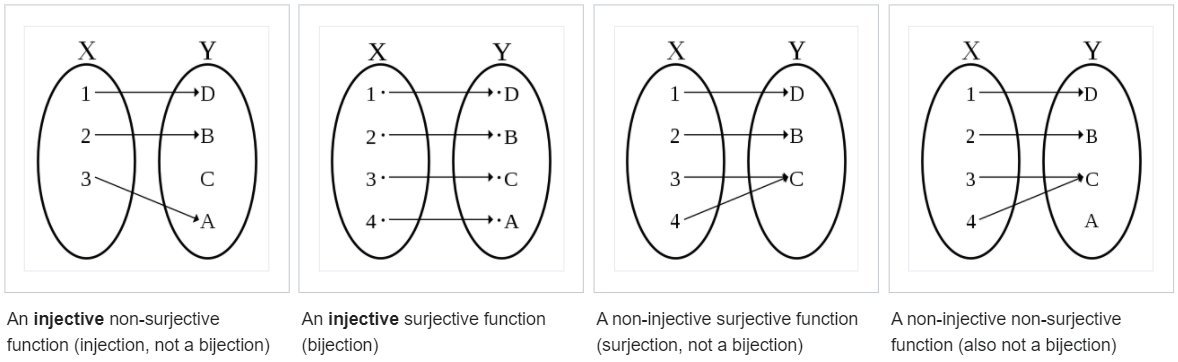
\includegraphics[width=\textwidth]{attachments/2.1-functions.png}
                \caption{From \href{https://en.wikipedia.org/wiki/Bijection}{Wikipedia}}
            \end{figure}
        
        \subsection{Equicardinality}
        
            \textbox{
                \begin{definition}[Equicardinality]
                    Two sets are \textbf{equicardinal} if there exists a bijective function that maps one to the other.
                \end{definition}
            }
            
            \begin{exercise}
                Are set of all natural numbers $\N$ and the set of all even numbers equicardinal? What about the naturals and odd numbers?
            \end{exercise}
        
    
    \section{Countability and infinite sets}
    
        \subsection{Countable sets}
        
            \textbox{
            \begin{definition}
                A set is \textbf{countable} if it is either finite or equicardinal to $\N$. Otherwise, it is \textbf{uncountable.}
            \end{definition}
            }
            
            We call the cardinality of countably infinite sets $\aleph_0$ (``aleph null"). Both $\Z$ and $\Q$ are countable as they are equicardinal to $\N$.
            
            To show that the integers is countable, we can arrange the its elements in alternating order of negative and positive naturals:
            \begin{align}
                \Z
                = \{0, 1, -1, 2, -2, ...\}
                = \{z_0, z_1, z_2, z_3, z_4, ...\}.
            \end{align}
            
            Since this arrangement ensures all integers are captured by the pattern, we can assign a natural number to each integer with indexing.
            
            Similarly for the rationals, we can arrange them in such a way that can be exhausted, and therefore indexed. We group the fractions by the sum of the numerator and denominator in ascending order:
            \begin{align}
                \Q = \left\{\frac{0}{1}, \frac{1}{1}, \frac{1}{2}, \frac{2}{1}, \frac{1}{3}, \frac{2}{2}, \frac{3}{1}, \frac{1}{4}, \frac{2}{3}, \frac{3}{2}, ... \right\}
                = \left\{0, 1, \frac{1}{2}, 2, \frac{1}{3}, 3, \frac{1}{4}, \frac{2}{3}, \frac{3}{2}, ... \right\}
                = \left\{q_0, q_1, q_2, q_3, q_4, ... \right\}.
            \end{align}
        
            More generally, an infinite set is ``listable" if (and only if) it is countable.
            
            Other countable sets include those of all
            \begin{itemize}
                \item
                constructible numbers
                
                \item
                computable numbers: set of reals computable to arbitrary precision
                
                \item
                algebraic numbers: root solutions to polynomials
                
                \item
                finite strings of zeros and ones
                
            \end{itemize}
                
            
            
        \subsection{Uncountable sets}
            \href{https://www.youtube.com/watch?v=elvOZm0d4H0}{Georg Cantor} introduced the concept of countability and produced a famous proof that the set of all real numbers is \textbf{uncountable}.
            
            The cardinality of the reals is called $\aleph_1$ (``aleph one").
            
            Some other sets with this cardinality are:
            
            \begin{itemize}
                \item $\R \setminus \Q$, the difference between the reals and rationals
                
                \item
                The interval $[0, 1]$ (or any non-empty real interval)
                
                \item
                $2^{\N}$, the power set of the natural numbers (or any $\aleph_0$ set)
                
                \item
                $\{0, 1\}^{\infty}$, the set of all infinite-length strings of zeros and ones.
            \end{itemize}
            
            We can show that $\{0, 1\}^{\infty}$ is equicardinal to [0, 1] by representing them as the binary decimals:
            
            
            \begin{exercise}
                Show that the cardinality of $[0, 1]$ is equal to that of any interval $[a, b]$.
            \end{exercise}
            
            \begin{exercise}
                Show that $\R$ and $\R^+$ are equicardinal.
            \end{exercise}
            
            \begin{exercise}
                See appendix \eqref{app:interval-cardinalities} for proof that the intervals $[0, 1]$, $[0, 1)$, $(0, 1]$, and $(0, 1)$ are all equicardinal. Show that $[0, 1]$ is equicardinal to $\R$.
            \end{exercise}
    
    \appendix
    \section{Appendix}
        
        \subsection{Equicardinality of intervals}\label{app:interval-cardinalities}
        
        \textbox{
            \begin{proposition}
                The intervals $(0, 1)$ , $[0, 1)$, $(0, 1]$, and $[0, 1]$ are equicardinal.
            \end{proposition}
        }
        
        \begin{proof}
            We can show there exist bijective functions from $(0, 1)$ to $[0, 1), (0, 1],$ and $[0, 1]$ by Hilbert's Hotel. Let $H = \left\{\frac{1}{n} : n \in \N, n > 1 \right\}$.
            
            Define $f_1 : (0, 1) \to [0, 1)$ as
            \begin{align}
                f_1(x) = \begin{cases}
                    0,              & x = \frac{1}{2}
                    \\
                    \frac{1}{n-1},  & x \in \left\{\frac{1}{n} : n \in \N, n > 2\right\}
                    \\
                    x,              & x \not\in H.
                \end{cases}
            \end{align}
            
            Define $f_2 : (0, 1) \to (0, 1]$ as
            \begin{align}
                f_2(x) = \begin{cases}
                    1,              & x = \frac{1}{2}
                    \\
                    \frac{1}{n-1},  & x \in \left\{\frac{1}{n} : n \in \N, n > 2\right\}
                    \\
                    x,              & x \not\in H.
                \end{cases}
            \end{align}
            
            Define $f_3 : (0, 1) \to [0, 1]$ as
            \begin{align}
                f_3(x) = \begin{cases}
                    0,              & x = \frac{1}{2}
                    \\
                    1,              & x = \frac{1}{3}
                    \\
                    \frac{1}{n-2},  & x \in \left\{\frac{1}{n} : n \in \N, n > 3\right\}
                    \\
                    x,              & x \not\in H.
                \end{cases}
            \end{align}
            
        Each of these functions is a bijection. Then the open interval is equicardinal to each of the other type of interval, which means they are all equicardinal.
    \end{proof}

    \begin{thebibliography}{9}
        
        \bibitem{book-of-proof}
        Hammack, Richard, (2018). \emph{Book of Proof, third edition}. Richard Hammack. \url{https://www.people.vcu.edu/~rhammack/BookOfProof/}
        
        \bibitem{rayo-mit}
        Rayo, Agustin, (2020). \emph{About this class}, lecture. Paradox and Infinity. MIT Open Learning Library. \url{https://openlearninglibrary.mit.edu/courses/course-v1:MITx+24.118x+2T2020/course}
        
        \bibitem{tao-notes}
        Tao, Terence. (2003). \emph{Week 1}, lecture notes. Honors Analysis Math131AH. University of California, Los Angeles. \url{https://www.math.ucla.edu/~tao/resource/general/131ah.1.03w/}
        
        \bibitem{tao-book}
        Tao, Terence. (2016). \emph{Analysis I, third edition}. Springer Singapore.
        
        \bibitem{}
        Ben (https://math.stackexchange.com/users/32139/ben). (2012), \emph{How to define a bijection between $(0,1)$ and $(0,1]$?} math.stackexchange.com. \url{https://math.stackexchange.com/q/160750}

        
        
    \end{thebibliography}
    % \bibliographystyle{plain}
    % \bibliography{1-sets.bib}
    
    
\end{document}